\section{Introduction}

\label{Section: Introduction}
A key technique in large-scale image retrieval systems is hashing. Image hashing aims to represent the information of an image using a binary code (e.g.,\( \pm 1\)) for efficient storage and accurate retrieval \cite{L2H2009}. Recently, deep learning to hash has shown significant improvements due to its robust feature extraction capability \cite{luoSurveyDeepHashing2023,xiaSupervisedHashingImage2014}, which utilizes neural networks to map high-dimensional feature vectors (e.g., 1024 dimensions) into compact binary codes (e.g., 64 bits). However, a fundamental challenge in deep hashing arises from the discrete nature of quantization. The \(sgn\) function used to generate binary codes has zero gradients almost everywhere. This gradient vanishing issue means that standard first-order methods are ineffective in training deep hashing networks \cite{Cao2017HashNetDL}. Continuous relaxation methods have been explored to address this issue, but inevitably introduce \textbf{quantization error:} the discrepancy between the optimized continuous values and the final discrete values \cite{weissSpectralHashing2008}. 
\begin{figure}[ht]
\centering
\includegraphics[width=0.6\columnwidth]{papers_img/V_W_regularization.pdf}
\caption{The V-type (left) versus W-type (right) regularizations.}
\label{Fig: the W and V regularizations}
\vspace{-5
ex}
\end{figure}
To mitigate this issue, researchers have developed specialized regularization techniques \cite{caoDeepCauchyHashing2018,li2017deep,liuDeepSupervisedHashing}. Among them, W-type regularizations, such as \(| |z| - 1| \), have proven effective.
These regularizers impose sharp penalties to encourage variables towards binary values (e.g., $-1$ or $1$). Mathematically, this approach naturally formulates deep hashing as a nonconvex composite optimization problem\footnote{A formal definition of this problem is provided in \Cref{Section: Problem Reformulation}.}:
\begin{align}
\label{Eq: the general nonlinear composite problem in intro}
\min_{\bx \in \calX} \quad \frac{1}{n} \sumn f_i (\bx) + \sumn h(\bD_i(\bx)),
\end{align} where \(f_i\) and \(\bD_i\) are continuously differentiable and \(h\) is a proper and lower semi-continuous (l.s.c.) regularizer.
Regularization techniques are widely used in machine learning and deep learning to encourage desirable model structures \cite{Dropout2014,wen2016learning,NCR2018Survey}. Classic examples include the 
\(\ell_1\) norm to introduce sparsity \cite{tibshirani1996regression} and the \(\ell_2\) norm weight decay to prevent overfitting \cite{tikhonov1943stability}. In practice, researchers typically apply stochastic (sub)gradient methods (SGD) directly \cite{Kingma2014AdamAM,tieleman2012lecture} to optimize the objective, and deep hashing follows this paradigm as well \cite{Cao2017HashNetDL,hoeOneLossAll2021,wang2023deep}. This seemingly effective choice, however, frequently leads to suboptimal performance. The regularizer is often nonsmooth around some regions; using subgradients may result in slow convergence and oscillation.

A powerful tool to circumvent the nonsmoothness of a regularizer is via its proximal operator. Proximal-based methods thus offer a promising solution for composite optimization \cite{Parikh2013ProximalA}. For a regularized deep network with  \(\bD_i(\bx) = \bx\) in \eqref{Eq: the general nonlinear composite problem in intro}, stochastic proximal gradient methods (SPGD) have been extensively studied \cite{davis2020stochastic,wang2019spiderboost,xu2023momentum,Xu2019NonasymptoticAO,xuStochasticOptimizationDC2019}. Recently, \cite{Yang2020ProxSGD} has established global convergence of SPGD for the \(\ell_1\) regularized model and \cite{yun2021adaptive} has presented a unified adaptive SPGD framework with \(\calO(\varepsilon^{-4})\) complexity for l.s.c. regularizations. However, these excellent methods crucially rely on regularizers with tractable proximal solutions, such as the well-known soft-thresholding operator of \(\ell_1\) norm (\Cref{Fig: the W and V regularizations}(a)). 
In contrast, while the W-type regularization (\Cref{Fig: the W and V regularizations}(b)) admits a closed-form proximal operator \cite{bai2019proxquant}, their composition with neural network outputs (i.e., \(h(\bD_i(\bx))\), which is typically highly nonconvex, creates a computationally intractable subproblem. This renders  SPGD  impractical for the problem \eqref{Eq: the general nonlinear composite problem in intro}.
% \cite{chen2016computing}
% In contrast, the W-type regularization (\Cref{Fig: the W and V regularizations} right) is generally.  Its sharp nonconvexity, especially around zero, makes it hard to find closed-form solutions for its proximal subproblem, which results in computationally expensive evaluation. This makes conventional SPGD methods impractical for the problem \eqref{Eq: the general nonlinear composite problem in intro} where \(h\) is a W-type regularization.

In fact, the nonlinear composite form \(h(\bD_i(\bx))\) presents a unique requirement in deep hashing, as the application of regularization in this field fundamentally differs from that in standard networks.  We demonstrate this distinction by comparing with a basic classification task in \Cref{Fig:comparison_classification_vs_hash}. While classification directly employs network outputs for prediction, deep hashing requires generating binary hash codes for downstream retrieval tasks. This unique requirement leads to W-type regularization, which typically constrains the final network output rather than focusing on parameter properties. Therefore, it is necessary to explicitly consider the nonlinear composite form.

Recent works \cite{duchiStochasticMethodsComposite2018,hu2023non,wang2024complexity,ADMMNolinear2024} have addressed compositional structures similar to \eqref{Eq: the general nonlinear composite problem in intro}, which ensure either weak convexity of \(h(\bD_i)\) or convexity on \(h\).  Other studies \cite{bian2021stochastic,huang2019faster} focus on stochastic optimization with linear compositional structures. On the contrary, our model faces a more challenging scenario where \(h\) is nonconvex with a nonlinear composition that implies \(h(\bD_i)\) is not weakly convex. \cite{bolteNonconvexLagrangian2018} considers the problem \eqref{Eq: the general nonlinear composite problem in intro} in deterministic setting. They converted it to a constrained optimization problem and established an asymptotic convergence via the Lagrangian-based method. However, their analysis does not provide non-asymptotic complexity guarantees for the stochastic case in deep hashing.
\begin{figure*}[t]
    \centering
    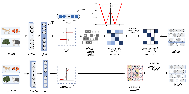
\includegraphics[width=0.95\textwidth]{papers_img/comparision_D2H_final.pdf}
    \caption{Comparison between deep learning for hashing and classification}
    \label{Fig:comparison_classification_vs_hash}
        \vspace{-4ex}
\end{figure*}
%\subsection{Motivation of nonlinear composite problem in deep hashing}
\subsection{Contributions}
In this paper, we propose an efficient deep hashing algorithm to address these challenges posed by nonlinear composition with W-type regularization. Our approach presents a reformulation of the W-type regularized problem using a decouple scheme and designs a new primal-dual algorithm using Fenchel duality. We aim to bridge the theoretical-practical gap by providing rigorous non-asymptotic convergence analysis and enhanced practical performance in deep hashing. Our main contributions are as follows:
\begin{itemize}[leftmargin=2em]
\item We reformulate deep hashing models with the W-type regularization into a two-block finite-sum optimization problem. This reformulation decouples the challenging $h(\bD(\bx))$, simplifying the sequential analysis.
\item Building on this problem, we propose \textbf{DualHash}, a stochastic primal-dual deep hashing algorithm. Using Fenchel duality, we partially transform the nonconvex W-type regularization optimization into a convex dual formulation that admits closed-form updates, ensuring robustness and stable convergence. To incorporate numerical acceleration, we develop two important instances: a momentum-based implementation (\textbf{DualHash-StoM}) and a variance-reduced implementation using StoRM (\textbf{DualHash-StoRM}).
\item We provide rigorous non-asymptotic complexity analysis for deep hashing optimization. Specifically, we establish an $\mathcal{O}(\varepsilon^{-4})$ complexity bound for DualHash-StoM and an improved optimal $\mathcal{O}(\varepsilon^{-3})$ complexity bound for DualHash-StoRM. Table~\ref{Table: summary of deep hashing algorithms} summarizes how our work compares to previous deep hashing methods. 
\item Extensive experiments on three standard datasets demonstrate the practical effectiveness of DualHash. In particular, our proposed method achieves consistently lower quantization errors across different bit lengths compared to baselines, validating the advantages of our primal-dual framework.
\end{itemize}
